\chapter{Fundamentals} % and theoretical background (BASICS)
\label{ch:fundamentals}

\section{Terms}
\label{sec:definitions}

The following is a list of definitions of common terms used in 3-dimensional computer graphics, topology (branch of mathematics), CAD and CAM. The definitions are partially based on lecture material \cite{mesh_basics, mesh_lecture10}.

\begin{description}
	
	\item[Solid] \hfill \\
	A solid is a object in 3-dimensional Euclidean space with a closed surface, separating space into two half-spaces.
	One is inside the solid, the volume of the solid, and the other outside.
	From a physical perspective, a solid is rigid and cannot be deformed, as opposed to \eg liquids.
	Examples of solids are cubes, pyramids, a flowerpot or your desk.
	
	
	\item[Triangulation/Tessellation] \hfill \\
	Although several representations exist to describe solids, \cf section \ref{sec:surface_representations}, triangle meshes are often preferred when exporting or distributing a solid.
	The process of converting an alternative representation to a triangle mesh is called triangulation or tessellation.
	\Eg, a common scenario in CAD is to export a model described using a CSG tree or dexel image as a triangle mesh.
	
	
	%\item[Chord error] \hfill \\
	%Tessellation is usually subject to a defined resolution.
	%Some solids such as spheres cannot be represented accurately by triangles.
	%The difference between the exact surface and the triangle approximation is called chord error.
	
	
	\item[Mesh] \hfill \\
	In 3-dimensional computer graphics, a mesh usually refers to a polygonal surface mesh:
	A mesh is a collection of faces, \ie polygons, edges between those faces, \ie lines, and vertices, \ie points in 3-dimensional space \cite{mesh_basics}.
	These mesh elements are described by the mesh's geometry and connectivity.
	Whereas the geometry simply specifies attributes of the vertices, the connectivity describes the complete topology, \eg edges connected to a vertex, face to vertices relationship, \etc.
	As a further aspect, the intersection between any pair of faces must be either a shared edge, a shared vertex or nothing \cite{mesh_lecture10}.
	In other words, faces can only connect to and not insect each other.
	%
	If a mesh is closed, it is a boundary representation, \cf section \ref{sec:surface_representations}, and therefore represents a solid.
	
	Another type of meshes are volumetric meshes, which also represent the contained volume in addition to the surface.
	Volumetric meshes are used, \eg, in finite element methods for physics simulations.
	
	
	\item[Manifold mesh] \hfill \\
	A mesh is a manifold, if it locally maps to Euclidean space.
	In other words, for each point on an n-dimensional mesh, the neighborhood of this point, \ie a region of the mesh, can be mapped to an Euclidean space of a dimension lower than n.
	This mapping must be bijective and is called homeomorphism or topological isomorphism.
	Each point of the region has a corresponding point in the mapped space and vice versa.
	In case of 3-dimensional meshes, a mesh is a 2-manifold if it can locally be mapped into 2-dimensional Euclidean space.
	\Eg the Earth is a 2-manifold as each local region can be mapped into a 2-dimensional plane, like the maps of an atlas.
	%
	Speaking strictly of triangle meshes, this restriction becomes concrete:
	A triangle mesh is a manifold if each edge is incident to only one or two faces and the faces incident to a vertex form an open or closed fan \cite{mesh_basics}.
	Figure \ref{fig:manifold} shows examples following and violating this requirements.
	
	\begin{figure}[H]
		\centering
		\begin{subfigure}[b]{0.3\textwidth}
			\centering
			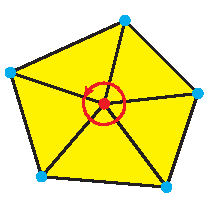
\includegraphics[width=\textwidth]{images/closed_fan}
			\caption{
				Manifold.
			}
			\label{fig:closed_fan}
		\end{subfigure}
		\begin{subfigure}[b]{0.3\textwidth}
			\centering
			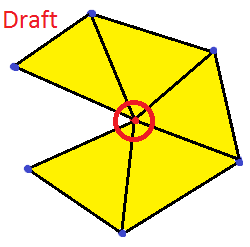
\includegraphics[width=\textwidth]{images/open_fan}
			\caption{
				Manifold.
			}
			\label{fig:open_fan}
		\end{subfigure}
		\\
		\begin{subfigure}[t]{0.32\textwidth}
			\centering
			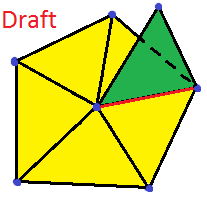
\includegraphics[width=\textwidth]{images/non_manifold_edge}
			\caption{
				Non-manifold.
			}
			\label{fig:non_manifold_edge}
		\end{subfigure}
		\begin{subfigure}[t]{0.32\textwidth}
			\centering
			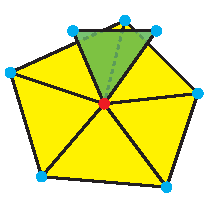
\includegraphics[width=\textwidth]{images/non_manifold_vertex}
			\caption{
				Non-manifold.
			}
			\label{fig:non_manifold_vertex}
		\end{subfigure}
		\begin{subfigure}[t]{0.32\textwidth}
			\centering
			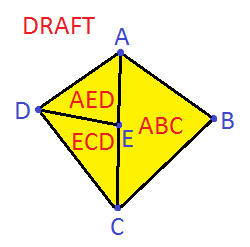
\includegraphics[width=\textwidth]{images/t_vertex}
			\caption{
				Non-manifold.
				}
			\label{fig:t_vertex}
		\end{subfigure}
		\caption{
			The upper images show a closed and opened fan of triangles incident to a vertex.
			Each edge is connected to only one or two faces.
			Both triangulations are 2-manifolds.
			%
			The bottom images show examples of not manifold meshes.
			The mesh in image \ref{fig:non_manifold_edge} contains an edge with three incident triangles.
			The mesh in image \ref{fig:non_manifold_vertex} contains a non-fan triangle connected to a vertex.
			Image \ref{fig:t_vertex} shows the T-vertex problem:
			Vertex $E$ lies directly on edge $AC$.
			There is either a degenerate triangle $AEC$ with zero area, or triangle $ABC$ should be a quadrilateral with $E$ and should be split along $EB$.
		}
		\label{fig:manifold}
	\end{figure}
	
	
	\item[Orientable mesh] \hfill \\
	Concerning the orientation of meshes, a few terms are defined \cite{mesh_basics}:
	The orientation of a single face is the cyclic order of its vertices.
	This order is also called winding order and determines the direction of the surface normal.
	The orientation of two adjacent faces is said to be compatible, if the two shared vertices on the shared edge are in opposite order.
	A mesh is orientable if it is a manifold and any pair of adjacent faces are compatible.
	Figure \ref{fig:orientable_mesh} shows examples of orientable and not orientable meshes.
	
	\begin{figure}[H]
		\centering
		\begin{subfigure}[b]{0.3\textwidth}
			\centering
			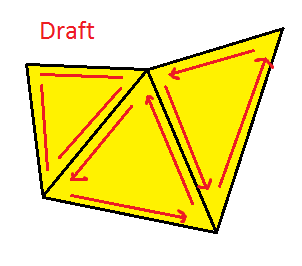
\includegraphics[width=0.8\textwidth]{images/orientable}
			\caption{Orientable mesh.}
			\label{fig:orientable}
		\end{subfigure}
		\begin{subfigure}[b]{0.3\textwidth}
			\centering
			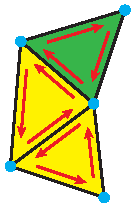
\includegraphics[width=0.8\textwidth]{images/not_orientable}
			\caption{Not orientable mesh.}
			\label{fig:not_orientable}
		\end{subfigure}
		\begin{subfigure}[b]{0.3\textwidth}
			\centering
			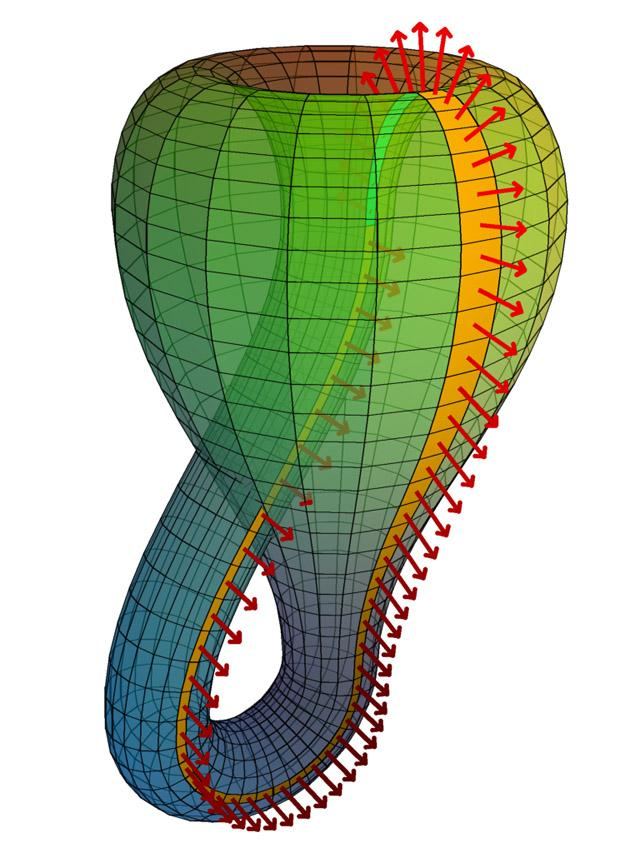
\includegraphics[width=\textwidth]{images/klein_bottle}
			\caption{The Klein bottle.}
			\label{fig:klein_bottle}
		\end{subfigure}
		\caption{
			The left and central image show an orientable and not orientable mesh.
			A mesh is orientable, if each pair of adjacent faces has a different vertex order on the shared edge.
			A famous example of a not orientable mesh is the Klein bottle on the right image, for which a strict inside and outside facing cannot be determined.
		}
		\label{fig:orientable_mesh}
	\end{figure}
	
	
	\item[Boundary] \hfill \\
	Edges of a mesh incident to only a face are called boundary edges.
	Vertices with an open fan of triangles are boundary vertices and connected to two boundary edges.
	A loop of connected boundary edges and vertices is called a boundary loop.
	
	
	\item[Closed/water-tight mesh] \hfill \\
	If a manifold mesh does not contain any boundary edges, which means that each vertex is part of a closed triangle fan, the mesh is a closed manifold.
	If a closed mesh is also orientable, it divides space into a half-space inside the mesh and one outside the mesh.
	The mesh is therefore a solid.
	The term water-tight is a common alias in CAM, meaning that a surface has no holes where water could enter or exit the solid represented by the mesh.
	
	
	%\item[Voronoi] \hfill \\
	
	
	\item[Delaunay triangulation] \hfill \\
	Named after the Russian mathematician Boris Delaunay, a 2-dimensional triangulation is called Delaunay when the circumcircle of each triangle does not contain a vertex of another triangle.
	The Delaunay triangulation is unique for each set of points as long as not more than three vertices lie on a circle. \Eg a quad can be triangulated along any of the diagonals to be Delaunay.
	The concept of 2-dimensional Delaunay triangulations can be extended to 3 dimensions, where each triangle of a manifold mesh has an empty circumscribing sphere.
	Such a triangle is sometimes also referred to as Gabriel 2-Simplex (G2S) \cite{g2s}.
	Delaunay triangulations produce very regular and visually appealing triangle meshes, as triangles with larger interior angles are preferred.
	Figure \ref{fig:delaunay_triangulation} shows a set of points with three different triangulations, with the first being Delaunay.
	
	\begin{figure}[H]
		\centering
		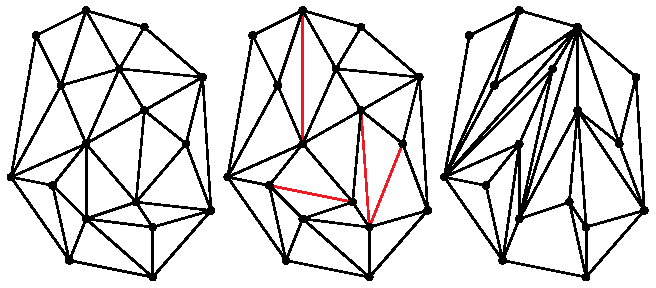
\includegraphics[width=0.9\textwidth]{images/delaunay_triangulation}
		\caption{
			Three different triangulations for the same set of points.
			Only the left one is a conforming Delaunay triangulation \cite{delaunay_image}.
		}
		\label{fig:delaunay_triangulation}
	\end{figure}
		
	
	\item[Stock] \hfill \\
	The stock is the original piece of material which is used as input for a milling machine.
	Material is removed from the stock using cutters to shape the stock into a desired form.
	This process is called subtractive manufacturing.
	In virtual machining, the stock is a solid.
	
	
	\item[Swept volume] \hfill \\
	In the context virtual machining, a single move of a cutting tool along a path is called a sweep.
	A swept volume is the volume which is covered by the cutting tool's solid during a sweep.
	The fast and efficient computation of such swept volumes for all kinds of paths, including self intersection, is still subject to research and discussed in the field of envelope theory.
	
	
	\item[Feature] \hfill \\
	In CAD, a feature is a local peculiarity of a mesh.
	Features are typically geometrically interesting aspects of a mesh which are typical for the represented surface.
	A cube for example has sharp edges and a fork has tines.
	These properties identify an object and are vital to recognize it as such.
	In terms of surface reconstruction, features are typically aspects of the represented object which are hard to reconstruct and require extended processing.
	Examples would be sharp edges and corners, small holes or thin structures.
	
\end{description}

\section{Surface representations}
\label{sec:surface_representations}

CAD and CAM software uses several different representations for final and intermediate solids and geometric parts like cutters, the manufactured workpiece or the current machining state.
The following section is based on a comprehensive overview with sketches and descriptions of the most commonly used representations in the area of virtual machining \cite{virtual_machining_review}. 

\begin{description}
	\item[Vector clipping] \hfill \\
	Vector clipping is mainly used in CAE to verify the correctness of a generated NC program before it is run on an actual milling machine.
	It was first described by Chappel \cite{vector_clipping} in 1983.
	The method requires the surface of the final workpiece as well as the stock.
	Initially, points on the final workpiece are calculated together with surface normals, \ie a point cloud, where the normals are not of unit length but long enough to reach the surface of the stock.
	To simulate the manufacturing process, the cutter is moved over this point cloud and the vectors attached to the points are clipped by the moving cutter, \cf figure \ref{fig:vector_clipping}.
	This method can be compared to a lawn mower, which cuts the grass, \ie the normal vectors, towards the ground, \ie the final workpiece.
	After cutting has completed, the lengths of the remaining vectors indicate the local error of the NC program.
	Vectors with positive lengths mark areas where too less material was removed and vice versa.
	The vector lengths are finally used to color the final workpiece where the color indicates the severity of the machining error.
	
	\begin{figure}[H]
		\centering
		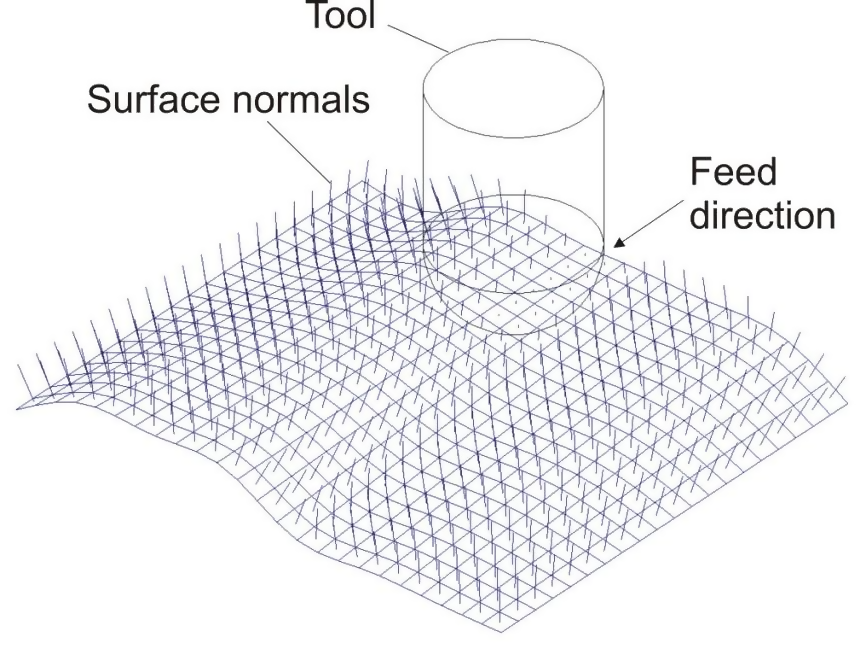
\includegraphics[width=0.5\textwidth]{images/vector_clipping}
		\caption{
			The vector clipping method \cite{virtual_machining_review}.
		}
		\label{fig:vector_clipping}
	\end{figure}
	 
	 
	\item[Z-maps and depth images] \hfill \\
	Describing solids using z-maps has been proposed by Anderson \cite{zmap} in 1978.
	It is furthermore the most widespread representation used in 3-axis material removal simulations.
	Z-maps approximate a solid by sampling its height at each crossing of a regular 2-dimensional grid.
	This grid is usually placed perpendicular to the cutting direction at one side of the stock, \eg the bottom.
	The volume of the z-mapped solid can be seen as the union of right square prisms where a prism is placed on each crossing of the grid with the height sampled at the crossing.
	Figure \ref{fig:zmap} shows such a prism approximation of a cuboid stock with a ball-end cutter removing material.
	As a z-map is a 2-dimensional scalar field with values at discrete regular positions, it can therefore be seen as an image, commonly referred to as depth image, \cf figure \ref{fig:depth_image}.
	
	Material is removed by creating a depth image for each cutter movement, \aka sweep, with the same position and orientation as the depth image of the workpiece.
	The sweep's depth image describes the removed material during the sweep.
	It is combined with the depth image of the workpiece by updating all depth values to be the minimum value of the workpiece's and sweep's depth image.

	Processing depth images can be greatly accelerated using GPUs as they contain special hardware for dealing with per-pixel depth information, \ie depth buffer or z-buffer.
	
	However, z-map representations have a fundamental drawback.
	As each depth value can only store the distance to a single surface points, z-maps cannot represent solids with a back-face or covered surfaces.
	
	\begin{figure}[H]
		\centering
		\begin{subfigure}[b]{0.4\textwidth}
			\centering
			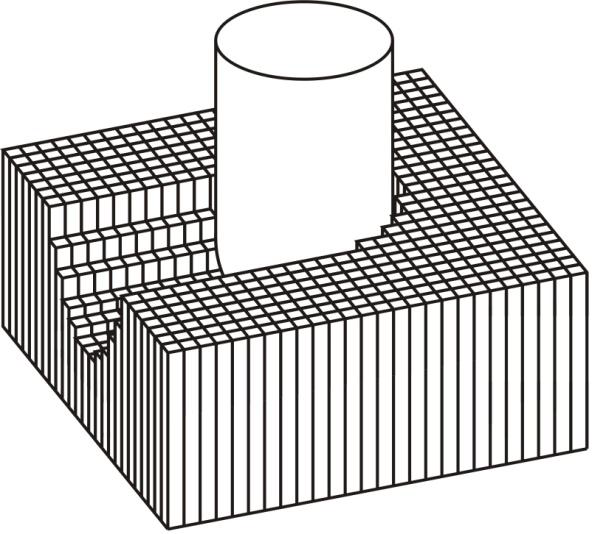
\includegraphics[width=\textwidth]{images/zmap}
			\caption{Z-map representation.}
			\label{fig:zmap}
		\end{subfigure}
		\begin{subfigure}[b]{0.4\textwidth}
			\centering
			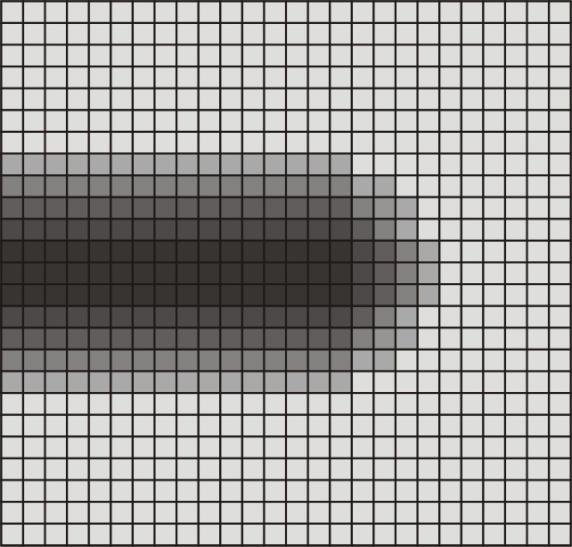
\includegraphics[width=\textwidth]{images/depth_image}
			\caption{Depth image.}
			\label{fig:depth_image}
		\end{subfigure}
		\caption{
			Representation of a cuboid stock with material removed using a ball-end cutter.
			The solid described by the z-map is represented using right square prisms in the left image.
			The z-map can be stored in a grayscale image as shown on the right  \cite{virtual_machining_review}.
		}
	\end{figure}
	

	\item[Dexel images] \hfill \\
	Dexel-based representations have been proposed by Hook to circumvent the shortcomings of depth images \cite{dexel}.
	Instead of a scalar value per pixel of a regular 2-dimensional grid, z-maps, a complex data element is stored, called a dexel, abbreviated from depth element.
	A dexel is created by tracing a ray, starting at a grid point, perpendicular to the grid's plane through the workpiece and collecting all surface intersections.
	Therefore, a 2-dimensional dexel image is sometimes also referred to as ray-rep, abbreviated from ray representation.
	Each dexel stores a sorted list of these intersections, where an intersection is also called a dexel node.
	A node basically contains the depth value of the intersection and can contain further informations such as a surface normal or a color value.
	Pairs of dexel nodes where the first node has been an entry and the second an exit are called segments and always lie inside the workpiece.
	Figure \ref{fig:dexel_image} shows a dexel representation of a half sphere with a smaller, concentric half sphere drilled out.
	
	Material removal is done in a similar fashion as with with z-maps.
	A dexel image is created for a sweep and then combined with the dexel image of the current workpiece.
	Instead of updating to the minimum value as done with z-maps, a 1-dimensional boolean subtraction of all sweep dexels from the workpiece dexels is performed.
	
	In comparison with image-based representations like z-maps and depth images, dexel-based approaches are able to represent overlapping surfaces and workpieces with a front- and a back-face.
	Nevertheless, the sampling resolution from the surface's perspective is dependent on the orientation of the surface towards the dexel grid.
	The more parallel the surface is to the grid, the smaller becomes the distance between two neighboring entry/exit points on the surface.
	In case the surface is perpendicular to the grid, the dexels lie parallel to the surface and do not capture any intersections.
		
	\begin{figure}[H]
		\centering
		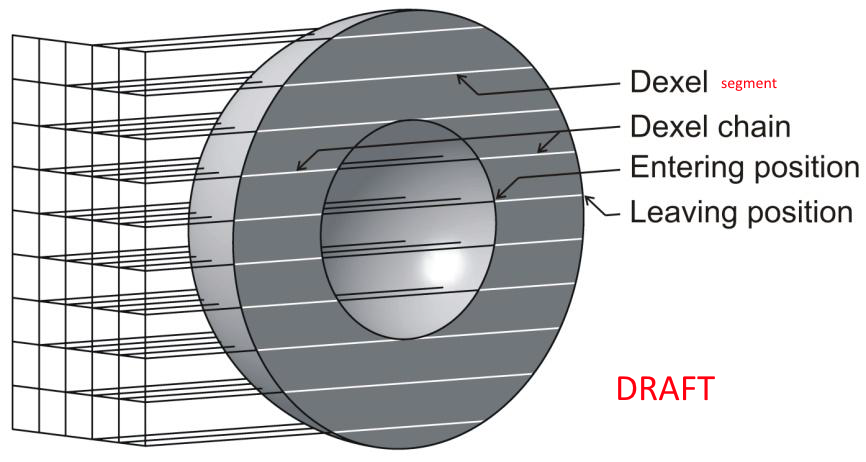
\includegraphics[width=0.8\textwidth]{images/dexels}
		\caption{
			Dexel image of a half sphere with a smaller, concentric half sphere drilled out \cite{virtual_machining_review}.
		}
		\label{fig:dexel_image}
	\end{figure}
		
		
	\item[Multi-dexel images] \hfill \\
	To increase the accuracy of dexel-based models, especially in regions of the surface where the surface normals are parallel to the dexels, multiple dexel images can be used.
	This idea was described by Benouamer \etal in 1997 to provide a good representation that can combine BRep and CSG models \cite{tridexel_intersection}.
	Although multiple dexel images can be created from any orientations, it is common to create three dexel images along the three axes of a Cartesian coordinate system.
	Therefore, the 2-dimensional dexel grids lie in the three planes defined by pairs of the coordinate system's axes, \ie xy-, yz-, zx-plane.
	This case of multi-dexel image is also referred to as triple- or tri-dexel image.
	Figure \ref{fig:tri_dexel_image} shows a triple-dexel representation of an octant of a centered unit sphere.
	
	\begin{figure}[H]
		\centering
		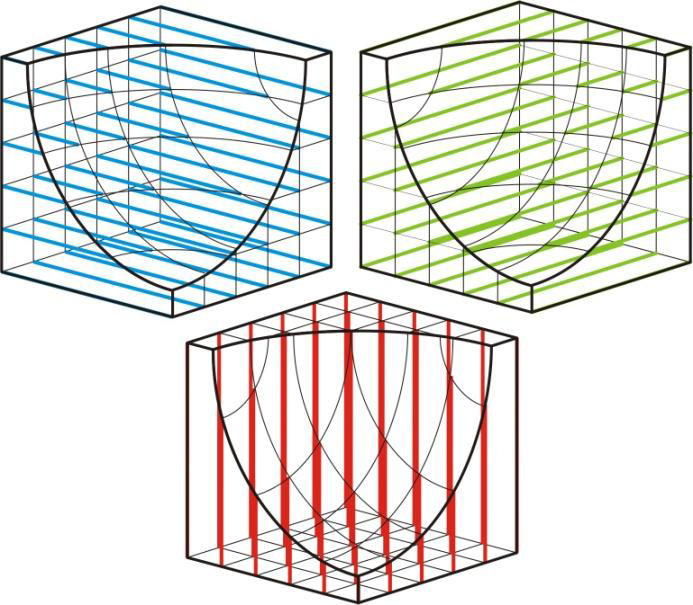
\includegraphics[width=0.8\textwidth]{images/tridexels}
		\caption{
			Tri-dexel images of an octant of a centered unit sphere.
			The left, blue image shows dexels along the x-axis, the centered, red image along the z-axis and the right, green image along the y-axis \cite{virtual_machining_review}.
		}
		\label{fig:tri_dexel_image}
	\end{figure}


	\item[Constructive Solid Geometry (CSG)] \hfill \\
	CSG is a technique widely spread in solid modeling.
	It has its origins in 1978 where Gossard \etal tried to use set theory to verify material removal in NC processes \cite{csg}.
	CSG describes a solid by its construction process from a set of simple primitives, making it therefore an interesting approach in procedural modeling.
	Although primitives are typically basic shapes such as cubes, spheres or cylinders, they can, in theory, be any kind of complex shape.
	Pairs of primitives can be combined using boolean set operations such as union, intersection or difference.
	The result of such an operation is a new solid, which can be again combined with other models or further primitives.
	A good visualization of these combinations is as a tree as shown in figure \ref{fig:csg_tree}.
	
	In virtual machining, material removal can be described as iteratively subtracting a new solid corresponding to the swept volume of the cutter during a single movement.
	Additive manufacturing, e.g. 3-dimensional printing, is also easily representable by adding a new solid.
	
	CSG trees can also be rendered directly using OpenGL or DirectX by making use of the GPU's depth and stencil buffers.
	Well known algorithms in this area include Goldfeather's algorithm \cite{goldfeather} and Nigel's Sequenced Convex Subtraction (SCS) algorithm \cite{scs}.
	
	\begin{figure}[H]
		\centering
		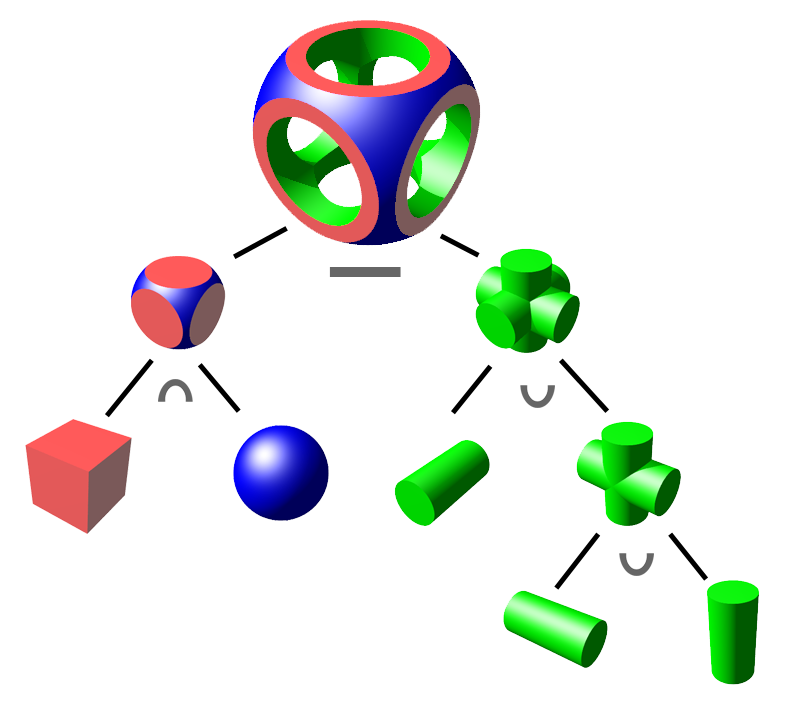
\includegraphics[width=0.8\textwidth]{images/csg_tree}
		\caption{
			A solid object modeled using CSG.
			The final shape of the object at the top is the result of combining the primitives at the bottom using boolean operations \cite{csg_tree}.
		}
		\label{fig:csg_tree}
	\end{figure}
	
	\item[Spacial decomposition] \hfill \\
	The volume covered by a solid can also be represented by listing regions in 3-dimensional space which are occupied by the volume.
	This representation is also commonly known as spacial occupancy enumeration.
	To enumerate occupied regions, one must first decompose space into smaller regions.
	This can be done in a uniform or hierarchical manner.
	
	Uniform spacial decomposition (USD) divides space into equally sized cells.
	An example would be a regular grid with cubic cells.
	This special case is known as voxel model, where a voxel, abbreviated from volume element, is a single cell of the regular grid.
	Figure \ref{fig:spatial_decomposition_usd} shows a voxel model of a simple solid.
	
	USDs are simple to create and implement as they only require a three dimensional grid which stores for each cell whether it is occupied or not.
	Boolean operations are also easily solved, as two uniform grids can be combined on a per cell basis similar to z-maps.
	However, USDs are highly memory demanding to achieve a sufficient resolution to accurately represent a solid.
	Furthermore, a high resolution may only be needed in certain regions of the solid, \ie features.
	
	Hierarchical spacial decomposition (HSD) overcomes the shortcomings of USDs.
	HSDs partition space in an adaptive way and increase their resolution only where detail is necessary.
	Therefore, HSDs usually require less memory at the cost of increased complexity.
	Figure \ref{fig:spatial_decomposition_hsd} shows an example of a solid represented by a hierarchically decomposed space.
	
	A common representative of HSDs are octrees.
	An octree on its highest level is a cube which is then recursively subdivided into eight half-sized cubes, \aka octants.
	This subdivision is only done, where a finer decomposition of space is necessary.
	Further examples of hierarchical decompositions are Binary Space Partitioning (BSP) and Bounding Volume Hierarchies (BVH).
	
	\begin{figure}[H]
		\centering
		\begin{subfigure}[b]{0.2\textwidth}
			\centering
			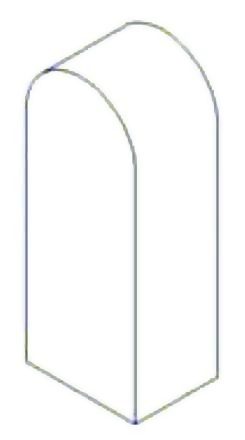
\includegraphics[width=\textwidth]{images/spatial_decomposition_solid}
			\caption{Solid}
			\label{fig:spatial_decomposition_solid}
		\end{subfigure}
		\begin{subfigure}[b]{0.2\textwidth}
			\centering
			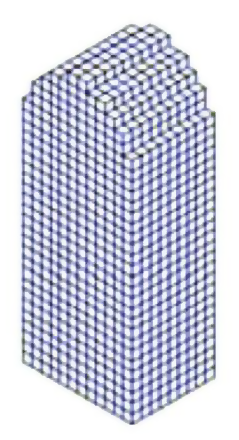
\includegraphics[width=\textwidth]{images/spatial_decomposition_usd}
			\caption{USD}
			\label{fig:spatial_decomposition_usd}
		\end{subfigure}
		\begin{subfigure}[b]{0.2\textwidth}
			\centering
			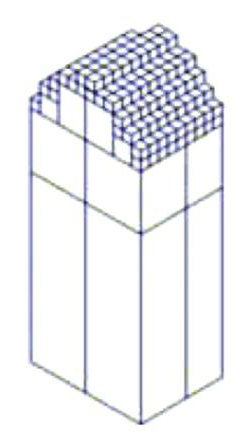
\includegraphics[width=\textwidth]{images/spatial_decomposition_hsd}
			\caption{HSD}
			\label{fig:spatial_decomposition_hsd}
		\end{subfigure}
		\caption{
			The solid on the left side can be described using spacial decomposition in either a uniform manner, central image, or a hierarchical manner, right image \cite{virtual_machining_review}.
		}
		\label{fig:spatial_decomposition}
	\end{figure}
	

	\item[Boundary representation (BRep)] \hfill \\
	Boundary representations, are the most wide-spread representations used in modern CAD systems.
	As the term suggests, BReps describe a solid by specifying its boundary surface.
	This surface typically consists of faces, \ie bounded surfaces, edges between those faces, \ie bounded curves, vertices, \ie 3-dimensional points, as well as their topology.
	BReps are therefore closed meshes.
	Faces can be specified using a variety of mathematical models from complex splines such as BSplines and NURBs to simple polygons like triangles.
	Figure \ref{fig:brep} shows an example of a BRep which represents a machining part using triangles as faces.
	%
	In the field of virtual machining, the faces of BReps are typically polygons which are connected by straight edges, \ie polyhedrons.
	The most common case are triangle meshes, although quadrilateral meshes are also popular in CAD.
	%
	Boolean operations like subtraction are hard to perform on arbitrary BReps.
	When considering only triangulated surfaces, the undertaking becomes doable, but still remains calculatively expensive and usually suffers from numerics.
	Boolean operations on triangulated BReps are typically available in modern CAD kernels.
	
	\begin{figure}[H]
		\centering
		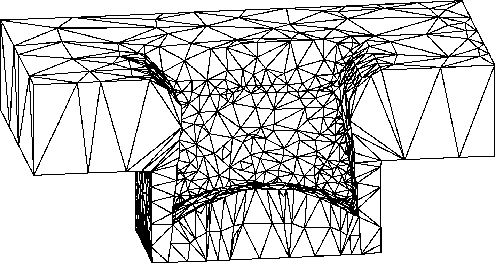
\includegraphics[width=0.8\textwidth]{images/brep}
		\caption{
			A boundary representation describes a machining part be specifying its boundary surface. A popular surface representation is a set of connected triangles \cite{virtual_machining_review}. 
		}
		\label{fig:brep}
	\end{figure}
	
	\item[Functional representation (FRep)] \hfill \\
	From a more mathematical point of view, surfaces can also be represented using real-valued functions.
	Pasko \etal give a good overview on this subject in the context of modeling and computer graphics \cite{frep}.
	\Eg a sphere is defined analytically as the infinite set of points with the same distance, \ie radius, to a distinct center point.
	By defining a function $d$ for the distance of a point $p$ to the center $c$ of a sphere $S$,
	\begin{align}
		d(p) &= \lvert c - p \rvert,
	\intertext{subtracting the radius $r$ and equating it with zero, a predicate}
		\mathit{on\_sphere}(p) &\Leftrightarrow d(p) - r = 0
	\intertext{is constructed that holds true for all points on the sphere's surface.}
	\intertext{More formally, $S$ is called a locus with regard to $\mathit{on\_sphere}$ and defined as}
		S &= \{\, p \in \mathbb{R}^3 \mid \mathit{on\_sphere}(p) \,\}.
	\end{align}
	Generalized, an object can be specified by classifying all spatial points using a continuous, real-valued function $f$. For each point $p \in \mathbb{R}^3$
	\begin{align}
		f(p) &> 0 \quad \text{if $p$ is inside the object,}               \notag \\
		f(p) &= 0 \quad \text{if $p$ is on the surface of the object and} \notag \\
		f(p) &< 0 \quad \text{if $p$ is outside the object.}              \notag
	\end{align}
	
	Functional representations excel in exactness, expressiveness and memory requirements.
	Additionally, some classes of problems are easier to solve on analytical models, \eg intersection tests.
	Furthermore, boolean operations and manipulations like bending and twisting are easier to formulate on mathematical entities then on the other data structures discussed in this section, \cf boolean operations on signed distance functions \cite{extended_marching_cubes}.
	
	Many primitives used in CSG are typically described using FReps.
	Several CAD kernels also use FReps internally to retain precision until the final result is exported, where it is typically tesselated into a BRep.
	
\end{description}
